\chapter{Implementierung}
\label{ch:Implementierung}

Grundlage für die Arbeit mit dem FPGA-Board ist eine Möglichkeit generierte Bitstreams auf das FPGA-Board zu übertragen.
Auf der Produkt-Seite des Herstellers des IceZero-Boards (Trenz Electronic)\cite{web:trenz_icezero}wird für diesen Zweck auf das Git-Repository des {\tt icotools}-Projekts verwiesen, in dem sich ein einfaches Testbeispiel zur Überprüfung des SRAM-Speichers befindet -- und das C-Programm {\tt icezprog} zum Flashen des Bitstreams.\\
Das {\tt icezprog}-Programm implementiert über direktes Ansprechen von GPIO-Pins (``bit-banging'') eine SPI-Schnittstelle zum Flash-Speicher des IceZero-Boards, und nach einem Neustart{\footnote{Der Neustart wird durch setzten des mit dem FPGA verbundenen GPIO-Pins ``CONFIG\_RESET'' ausgeführt} konfiguriert sich das FPGA selbständig mit dem Inhalt des auf dem Flash-Speicher abgelegten Bitstreams.\\
Für die spätere Verwendung des {\tt IcoSoc}-Projekts wird allerdings noch weitere Funktionalität benötigt. Wichtig ist hier vor allem die Möglichkeit Speicherinhalte mit einem ``Offset'' in den Flash-Speicher zu schreiben, da später zusätzlich zum Bitstream auch ein ``appimage'' auf dem Flash-Speicher abgelegt wird, das den auszuführenden C-Code für den {\tt IcoSoc} enthält.\\
Das {\tt icotools}-Projekt enthält mit dem Tool {\tt icoprog} ein Programm das (unter anderem) Offsets unterstützt und in erster Linie zum Programmieren von Bitstreams für das IcoBoard gedacht ist. IcoSoc unterstützt außerdem Debugging-Funktionalitäten die über eine eigene 10 Bit breite parallele Schnittstelle zum Raspberry Pi realisiert sind. Diese Schnittstelle kann auch verwendet werden um ein {\tt appimage} beim Start des IcoSocs direkt zu laden, ohne dass es vorher im Flash-Speicher abgelegt werden muss. Die Schnittstelle wird ebenfalls über das {\tt icoprog}-Tool angesprochen.\\
Um die selbe Funktionalität auch für das IceZero-Board zur Verfügung zu stellen wurde als erstes das {\tt icoprog}-Tool entsprechend angepasst. 

\section{Anpassung des Tools zum Programmieren des Bitstreams (icoprog)}
\label{ch:Implementierung:sec:icoprog}

Das IcoBoard verfügt wie das IceZero-Board über einen 40-Pin-Header zum Anschluss an ein Raspberry Pi. Davon abgesehen kann das IcoBoard aber auch mit einem zusätzlichen FTDI-Interfaceboard über USB programmiert werden. Das {\tt icoprog}-Programm enthält deswegen sowohl Methoden zur Programmierung via USB als auch über die GPIO-Pins des Raspberry Pis, und noch eine zusätzliche GPIO-basierte Variante für ein anderes Board. Ursprünglich war geplant eine Konfiguration für das IceZero-Board direkt in das icoprog-Tool zu integrieren, aufgrund der ohnehin schon unübersichtlichen Code-Basis wurden die benötigten Komponenten aber in ein eigenes Programm namens {\tt icozctl} ausgelagert, dass dann später um Funktionen zur Steuerung der Aufnahme und Datenübertragung erweitert wurde.\\ 
Für die Anpassung mussten einige GPIO-Pins geändert werden, da beim IceZero-Board nicht alle Pins der GPIO-Headers mit dem FPGA verbunden sind. (Das IcoBoard verwendet einen iCE40-Chip im CT256-Formfaktor, weswegen deutlich mehr Pins zur Verfügung stehen als beim IceZero-Board\cite{web:trenz_icoboard}).\\
Davon abgesehen ist auf dem IcoBoard ein zusätzlicher MachXO2-Chip von Lattice verbaut, der (unter anderem) das SPI-Signal vom Raspberry Pi je nach gesetztem Chip-Select-Signal entweder direkt an das FPGA oder den Flash-Speicher weiterleitet. Beim IceZero-Board sind das FPGA und der Flashspeicher direkt an die gleichen GPIO-Pins des Raspberry Pis angeschlossen (inklusive Chip-Select-Signal), ein gezieltes Ansprechen der einzelnen Komponenten ist deswegen nicht möglich, und die entsprechenden Chip-Select-Signale wurden aus dem Code entfernt. 
Im späteren Verlauf der Implementierung wurde entschieden die parallele Schnittstelle zu entfernen, da mit ihr keine bidirektional Kommunikation mit der nötigen Geschwindigkeit realisiert werden konnte. Stattdessen wurde mit den frei-gewordenen Pins eine SPI-Schnittstelle und ein zusätzlicher UART für einfache Debug-Ausgaben umgesetzt.\\
Ein direktes Flashen von {\tt appimages} beim Starten des IcoSoc ist dementsprechend bei aktuellem Stand nicht möglich und die erweiterten Debug-Funktionen des IcoSoc sind nicht verfügbar. 
Davon abgesehen kann das {\tt icozctl}-Tool auf dem IceZero-Board mit der gleichen Syntax wie {\tt icoprog} für das IcoBoard verwendet werden.
Zu Debug-Zwecken wurde {\tt icoprog} außerdem um eine Option ``-N'' erweitert, mit der ein Offset für das Auslesen des aktuellen Flash-Speicher-Inhalts angegeben werden kann.

\section{Portierung und nötige Anpassungen des Verilog-SoCs (IcoSoc)}
\label{ch:Implementierung:sec:icosoc}
Als nächstes wurde das IcoSoc-Projekt auf das IceZero-Board portiert. 

\subsection{Struktur des IcoSoc-Projekts}
Zum Überblick soll erst ein kurzer Blick auf die Verzeichnisstruktur des Projekts geworfen werden:
\begin{minted}{bash}
./common
./common/firmware.c
./common/firmware.S
./common/icosoc_debugger.v
./common/icosoc_raspif.v
./common/picorv32.v
./common/riscv_flash.ld
[...]
./examples
./examples/event_recorder
./examples/hello
[...]
./mod_gpio
./mod_rs232
./mod_spi
[...]
./README
./icosoc.py
\end{minted}

Im Verzeichnis {\tt common/} befinden sich die Grundbausteine des IcoSoc-Systems. Dazu gehört die Verilog-Implementierung des PicoRV32-Prozessors und weitere grundlegende Systemkomponenten wie zum Beispiel die erwähnte Raspberry Pi Schnittstelle (``raspif'') und außerdem die nötige Firmware zum Starten des IcoSocs und zum Laden der {\tt appimages}. Zusätzlich findet sich hier auch das benötigte Linker-Skript für den C-Code der {\tt appimages}.\\
Im Verzeichnis {\tt examples/} liegen verschiedene Beispiel-Projekte, unter anderem ein ausführliches ``Hello world''-Beispiel in dem die für IcoSoc-Projekte verfügbaren Komponenten vorgestellt werden -- und das in dieser Arbeit entworfene Event-Recorder Projekt.\\
Darauf folgen die verfügbaren IcoSoc-Module jeweils in einem eigenen Unterverzeichnis.\\
Das Modul ``mod\_gpio'' stellt zum Beispiel die Funktionalität zur Verfügung, das im C-Code GPIO-Pins als Ausgänge definiert werden können und ihr Ausgangspegel anschließend über das Schreiben an eine bestimmte Speicheradresse gesetzt werden kann. 
Zuerst muss das Modul in der Projekt-Konfigurationsdatei {\tt icosoc.cfg} aktiviert werden:
\begin{minted}{python}
board icoboard
mod gpio gpios
    address 2
    connect IO pmod2 pmod1
\end{minted}

Die Benutzung im C-Code würde dann folgendermaßen aussehen:

\begin{minted}{c}
// Alle GPIO Pins als Ausgang verwenden
icosoc_gpios_dir(0xffff);

// Ersten Pin auf '1' setzen
icosoc_gpios_set(0x0001);
\end{minted}

Wobei der ``set''-Befehl des Moduls als einfacher Schreibbefehl an eine Speicheradresse implementiert ist:
\begin{minted}{c}
static inline void icosoc_@name@_set(uint32_t bitmask) {
    *(volatile uint32_t*)(0x20000000 + @addr@ * 0x10000) = bitmask;
}
\end{minted}

Die Module selbst sind in Verilog geschrieben und bilden somit eine Brücke zwischen dem Timing-stabilen Verilog-Teil und dem langsameren C-Code.\\

Direkt im Projekt-Verzeichnis findet sich eine README-Datei und das Python-Skript {\tt icosoc.py}.
Das Python-Skript generiert aus der Projekt-Konfigurationsdatei mithilfe der verfügbaren Module und Grundkomponenten den eigentlichen Verilog-Code für den IcoSoc und kümmert sich um die ordnungsgemäße Verbindung und Konfiguration der Module. (Die Platzhalter ``@name@'' und ``@addr@'' in der Definition der {\tt gpio\_get()}-Methode werden hier zum Beispiel auch durch die in der Konfigurationsdatei festgelegten Werte ersetzt).
Zusätzlich wird ein {\tt Makefile} generiert, mit dem das Projekt synthetisiert, der C-Code kompiliert, und abschließend der erzeugte Bitstream und das {\tt appimage} auf das FPGA-Board geflasht werden können.

\subsection{Portierung des IcoSoc-Projekts}

Für die Portierung waren gemäß der Struktur des IcoSoc-Projekts hauptsächlich Anpassungen im {\tt icosoc.py} Skript nötig.\\
Das Python-Skript generiert unter anderem auch die {\tt icosoc.pcf}-Datei, in der die Pin-Definitionen für die Synthese festgelegt werden.
Da auf dem IceZero-Board ein anderes iCE40-FPGA-Modell verwendet wird, mussten hier alle Pin-Definitionen gemäß den Informationen aus dem IceZero-Board-Schaltplan\cite{doc:schematic} angepasst werden.
Ein einfaches Beispiel wäre der Eingang des Systemtakts und die LED-Pins: 
\begin{minted}{python}
if board == "icezero":
    icosoc_pcf["10-std"].append("""
    set_io CLKIN  49  // icoboard: R9
    set_io LED1   110 // icoboard: C8
    set_io LED2   93  // icoboard: F7
    set_io LED3   94  // icoboard: K9
[...]
""")
\end{minted}

Wie im Beispiel ersichtlich ist wurden die meisten durchgeführten Änderungen mit der Variable ``board''  parameterisiert, so dass die Unterstützung mehrerer Board mit vergleichsweise geringem Aufwand möglich wäre\footnote{Für die Untersützung mehrerer Boards wäre eine tiefergehende Umstrukturierung des IcoSoc-Projekts sinnvoll, die aber über den Umfang dieser Arbeit hinausgeht}.

Die PMOD-Pins werden den verwendeten Modulen nach Bedarf zugewiesen und nach einem festen Namensschema benannt (siehe hierzu auch ``\nameref{sec:pmod_all}'').\\
Auch hier wurden die entsprechenden Pin-Definitionen angepasst.\\
Für IcoSoc-Module sind grundsätzlich nur Verbindungen zu PMOD-Pins vorgesehen. Für die geplante Funktionalität werden allerdings auch Verbindungen zu anderen FPGA-Pins und Verilog-Signalen (wie zum Beispiel dem CLKIN Pin) benötigt. Das Skript wurde so angepasst, dass Moduldefinitionen auch andere -- in einer Liste festgelegte --  Signale verwenden dürfen.
\begin{minted}{python}
def make_pins(pname):
    [...]
    allowed_signals = ['CLKIN']
    if pname in allowed_signals:
        return [pname]
    [...]
\end{minted} 

Wie schon erwähnt wurde außerdem die ``RASPIF''-Schnittstelle entfernt, und stattdessen ein einfacher UART für Debug-Ausgaben integriert.\\
Die Änderungen wurden analog zu einem {\tt icotools}-Fork\footnote{Der Fork enthält außerdem zusätzliche Beispiel-Projekte und unter anderem ein I$^2$C-Modul} auf Github durchgeführt, bei dem die gleichen Anpassungen für ein anderes iCE40-basiertes Board durchgeführt wurden (``BlackIce II''-Board, siehe \cite{web:lawrie_fork}). \\
Davon abgesehen wurde ein unbenutztes ``HRAM''-Signal aus dem Design entfernt und kleinere Änderungen an der Generierung des Makefiles durchgeführt. Der {\tt icoprog}-Befehl wurde durch {\tt icozctl} ersetzt und das Log-Level wurde auf die Stufe ``-v2'' reduziert. Außerdem muss dem Place-and-Route-Befehl ({\tt arachne-pnr}) und der durchgeführten Timing-Analyse ({\tt icetime}) mit der Option {\tt -P tq144:4k} der Formfaktor des iCE40-Chips mitgegeben werden, damit die Pindefinitionen richtig zugeordnet werden können.   
Mit den genannten Änderungen liegt ein voll funktionsfähiger Port des IcoSoc-Projekts für das IceZero-Board vor.

\section{Implementierung des Event-Recorder Moduls}
\label{ch:Implementierung:sec:Event-Recorder}

Zur Implementierung der Signalerfassung wurde ein eigenes IcoSoc-Modul namens {\tt mod\_triggerrec} erstellt.
\subsection{GPIO-Eingänge}
Die Erfassung der an den PMOD-Headern anliegenden Eingangssignale erfolgt analog zum GPIO-Modul, allerdings mit dem Unterschied dass die verwendeten Pins fest als Eingänge definiert werden.
Dafür wird bei der Instantiierung des SB\_IO-Primitves für den PIN\_TYPE die Bit-Kombination {\tt 0000\_01} gesetzt (siehe ``Input Pin Function Table'' aus der SiliconBlue ICE Technology Library\cite[S.~73]{doc:tec_lib}).\\ 
Auf den Registerinhalt des so definierten SB\_IO-Primitives kann dann in Verilog mit einem einfachen ``wire'' der entsprechenden Bit-Breite zugegriffen werden:
\begin{minted}{verilog}
// gpio input
wire [IO_LENGTH-1:0] io_in;
\end{minted}

\subsection{Bus-Schnittstelle}
Um Daten aus dem Verilog-Teil in den C-Teil transferieren zu können muss die Bus-Schnittstelle des IcoSoc in Verilog implementiert werden.
Dafür werden -- wie im GPIO-Modul -- die Signale {\tt ctrl\_rd}, {\tt ctrl\_wr}, {\tt ctr\_addr} und {\tt ctrl\_wdat} als Eingänge {\tt ctrl\_rdat} und {\tt ctrl\_done} als Ausgänge des Moduls zur Verfügung gestellt.
Die Bus-Schnittstelle wird (vereinfacht) folgendermaßen umgesetzt:
\begin{minted}{verilog}
always @(posedge clk) begin		
	if (!ctrl_done) begin
		ctrl_done <= 1;
		// write from bus to local register associated with address 4
		if (|ctrl_wr) begin
			if (ctrl_addr == 4) local_register <= ctrl_wdat;
		end
		// read from local registers to bus
		if (ctrl_rd) begin
			if (ctrl_addr == 4) ctrl_rdat <= local_register;
		end
	end
end
\end{minted}

Für die meisten Register wird eine Länge von 64 Bit verwendet. Da der Bus eine Breite von 32 Bit hat (also nur 32 Bit in einem Takt übertragen kann), wird für diese Register eine zusätzliche Zustandsvariable ({\tt ctrl\_state}) verwendet, so dass beim ersten Zugriff immer die höheren 32 Bit übertragen werden und beim zweiten Zugriff (und zweiten Zustand) die unteren 32 Bit.. 

\subsection{BRAM-Speicher für die Event-Definitionen}

Da aus dem Verilog-Modul ein direkter Zugriff auf die Event-Definitionen und -Trigger möglich sein soll werden diese in einem Register-Array abgelegt.\\
Die Länge des Arrays ist parametrisiert, so dass die Anzahl der gewünschten Event-Trigger bei der Synthese angegeben werden kann. Bei einfacher Lese- und Zugriffs-Logik wird das Array als BRAM synthetisiert wird, und es werdem damit keine zusätzlichen `Logic Slices' in Anspruch genommen.\\  
Im Trigger-Array werden die 64 Bit langen Event-Definitionen jeweils in zwei aufeinander-folgende 32-Bit Werte aufgeteilt, da dies die Bus-Logik etwas vereinfacht.  
Bei der Bus-Kommunikation wird die angeforderte Adresse ({\tt ctrl\_addr}) mit einem Offset\footnote{Die Adresse hat um der Bitbreite der Registerelemente zu entsprechen einen ``Multiplikator'' und wird deswegen zusätzlich per Rechts-Shift verkleinert bevor der Index generiert werden kann} in den Index des Event-Registers-Arrays umgesetzt, so dass alle Array-Elemente direkt vom Bus ansprechbar sind. 

\subsection{Erkennung von Signaländerungen und Events}

Der erste Schritt bei der Auswertung des GPIO-Registers ist die kontinuierliche Erkennung von Signaländerungen.\\
Dies wird im Verilog-Code durch einen einfachen Vergleich und ein Zwischenspeichern des alten Signalzustands erreicht:

\begin{minted}{verilog}
	// input capture
	always @(posedge clk_fast) begin
		// increment counter if active
		if (status[0])  
			counter <= counter + 1;
		
		// on input changes ..
		if ((io_buf2 != io_buf1)) begin
			data_in_fast <= { io_buf1, 1'b0, counter[46:0] };
			shift_in_fast <= 1;
		end
	end
	
	io_buf1 <= io_in;
	io_buf2 <= io_buf1;	
	[...]

\end{minted}
An dieser Stelle wird auch der Zähler erhöht, wenn das Modul in aktiviertem Zustand ist.\\
Darüber hinaus wurde auch eine Event-Erkennung in Verilog begonnen. Bei der vorhandenen Implementierung wird bei der Synthese allerdings eine große Menge kombinatorischer Logik generiert, und es können nicht ausreichend viele Event-Definitionen umgesetzt werden (Die Kapazität des iCE40-Chips wird bei circa 8 Event-Definitionen erreicht, bei großer Auslastung der Logic Slices erhöhen sich auch die Place-and-Route-Zeiten auf Werte von einer halben Stunde oder mehr). \\
Ohne weitere Optimierungen ist die Event-Erkennung in Verilog deswegen nicht praktikabel und wurde bei aktuellem Stand der Arbeit wieder deaktiviert.\\
Es ist anzumerken, dass die Erkennung von Signaländerungen das Datenvolumens bei der Aufnahme bereits stark reduziert -- insbesondere bei geringer Signaldichte.

\subsection{Cross-Clock BRAM-Puffer}

Da die Event-Erkennung im Verilog-Teil noch nicht abgeschlossen ist, aber auch um schnell aufeinander-folgende Signale ohne Verlust erfassen zu können, macht es Sinn bereits direkt auf dem FPGA ein Puffer für die Aufnahmedaten zu implementieren. Der Puffer soll wiederum als BRAM synthetisiert werden, da es sich um größere Datenmengen handelt und keine kombinatorische Logik verbraucht werden soll.\\
Bei FPGA-Implementierungen werden derartige Puffer häufig benötigt -- und dabei oft mit der zusätzlichen Funktionalität, dass Daten zwischen unterschiedlich schnell getakteten Komponenten ausgetauscht werden. Der Austausch von Daten zwischen verschiedenen Taktdomänen ist dabei kein triviales Problem. Das {\tt IcoSoc}-Projekt enthält in der Datei {\tt icosoc\_crossclockfifo.v} allerdings bereits eine Implementierung eines solchen Cross-Clock-Puffers, die für das {\tt raspif}-Modul verwendet wird. Da keine weitere Dokumentation zum Puffer-Modul vorhanden ist, wurde zuerst eine {\tt iverilog}-Testbench geschrieben, die die erwartete Funktionsweise bestätigt hat. Das {\tt crossclockfifo}-Modul konnte so erfolgreich als BRAM-Puffer in das Event-Recorder-Modul eingebunden werden.\\
IcoSoc-Module laufen im Normalfall mit dem Systemtakt des IcoSocs. Dieser wird durch eine PLL-Konfiguration generiert und liegt bei (circa) 20 Mhz.\\
Zusammen mit der bei der Portierung des {\tt IcoSoc}-Projekts durchgeführten Anpassung, dass IcoSoc-Module auch andere Ein- und Ausgänge als die PMOD-Pins haben können, konnte so das 100 Mhz schnelle CLKIN-Signal an das Event-Recorder-Modul weitergereicht werden und damit eine Steigerung der Erfassungsgeschwindkeit auf 100 Mhz erreicht werden.  

\subsection{Simulation des Event-Recorder-Moduls mit iverilog}

Das Verhalten des Event-Recorder-Moduls lässt sich mit einer {\tt iverilog}-Testbench simulieren.\\
Durch die Bus-Schnittstelle kann dabei die erwartete Funktionalität geprüft werden ohne die anderen Komponenten des {\tt IcoSoc}-Systems mitsimuliert werden  müssen.

In der Testbench werden zwei ``tasks'' für den schreibenden und lesenden Bus-Zugriff erstellt, deren Verhalten einem tatsächlichen Bus-Zugriffs entspricht:

\begin{minted}{verilog}
	task ctrl_write(input [15:0] addr, input [31:0] data); begin
		ctrl_wr <= 1;
		ctrl_rd <= 0;
		ctrl_addr <= addr;
		ctrl_wdat <= data;
		@(posedge clk);
		while (!ctrl_done) @(posedge clk);
		ctrl_wr <= 0;
	end endtask

	task ctrl_read(input [15:0] addr); begin
		[...]
	end endtask
\end{minted}

Anschließend können in der Testbench Speicher-Zugriffe -- analog zu den vom Modul definierten C-Funktionen -- simuliert werden und ihr Ergebnis geprüft werden.
\begin{minted}{verilog}
		// test write to status register (address 0x04)
		ctrl_write('h4, 'h01); 
		repeat (2) @(posedge clk);
		
		// read status register
		ctrl_read('h4);	
		repeat (2) @(posedge clk);
		
		$display("Status: %s", (ctrl_rdat == 'h01)? "OK" : "Not OK");                                                    //$	

\end{minted}

Für die Ausführung der Testbenches ist jeweils ein kurzes Bash-Skript vorhanden, so kann im Modul-Verzeichnis {\tt mod\_triggerrec} zum Beispiel der Befehl
\begin{minted}{bash}
sh testbench.sh
\end{minted}
ausgeführt werden, und die erzeugte VCD-Datei mit {\tt gtkwave} geöffnet werden:
\begin{minted}{bash}
gtkwave testbench.vcd
\end{minted}

Der folgende Auszug zeigt zum Beispiel einen Signalübergang von `0' auf `1' am ersten Pin des Event-Recorders, wobei der Signal-Wert (0x0001) und der entsprechende Zähler-Wert (0) über das Register {\tt data\_in\_fast} in den Cross-Clock-FIFO übertragen werden. Es folgt ein Bus-Zugriff auf die Adresse 0x0C, bei dem der im FIFO gespeicherte Wert abgefragt und über das Register {\tt data\_out} an den Bus übertragen wird. Der Lese-Zugriff erfolgt in zwei Einzelschritten, bei den zuerst die oberen und dann die unteren 32 Bit übertragen werden (siehe {\tt ctrl\_stat} und {\tt ctrl\_done}-Signal). \\
(Der Signalübergang wird in der Simulation auch als Start-Event erkannt, weswegen der Zähler erst nach dem Signalwechsel aktiv wird). 
\begin{figure}[H]
	\centering
	\captionsetup{justification=centering,margin=2cm}
		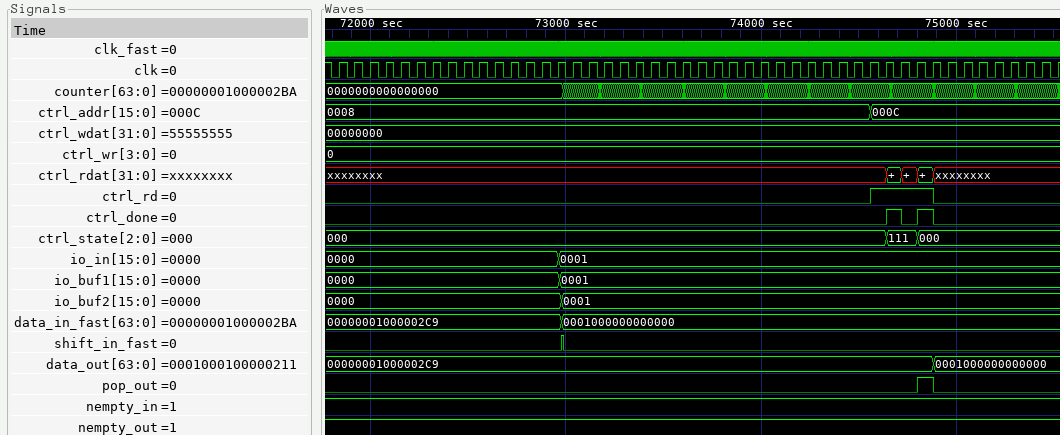
\includegraphics[width=\textwidth]{../figures/simulation_data_in.png}
		\caption[Auszug aus der Simulation des Event-Recorder-Moduls]{Auszug aus der Simulation des Event-Recorder-Moduls}
	\label{fig:ice40_pmod_pins}
\end{figure}

\section{Implementierung eines SPI-Slave-Moduls}
\label{ch:Implementierung:sec:SPI-Slave}

Für den Austausch der Daten mit dem Raspberry Pi wird noch eine weitere Komponente für die SPI-Kommunikation benötigt. Diese Komponente soll wieder als {\tt IcoSoc}-Modul umgesetzt sein, um die Ausführung des C-Codes nicht unnötig zu verlangsamen. Das {\tt IcoSoc}-Projekt enthält bereits ein SPI-Modul, allerdings handelt es sich hier um eine reine Master-Implementierung (vor allem zum Ansprechen externer Hardware wie zum Beispiel kleinerer LCDs). 
Deswegen wurde noch ein zusätzliches SPI-Slave-Modul entworfen.\\
Die Bus-Logik funktioniert analog zum Event-Recorder-Modul, wobei im C-Teil eine ``bidirektionale'' Übertragungsfunktion zur Verfügung gestellt wird. Es wird ein 32-Bit-Wert als Argument übergeben und gleichzeitig einen 32-Bit-Wert als Rückgabe geliefert. 
\begin{minted}{c}
static inline uint32_t icosoc_@name@_xfer(uint32_t value)  
{
    *(volatile uint32_t*)(0x20000004 + @addr@ * 0x10000) = value;
    return *(volatile uint32_t*)(0x20000008 + @addr@ * 0x10000);
}
\end{minted}
Das Argument sind dabei die über SPI zu sendenden Daten, und der Rückgabewert die empfangenen Daten.\\
Der SPI-Transfer ist dabei ähnlich einem Schieberegister implementiert, bei dem bei jeder steigenden Taktflanke ein Bit der Sende-Daten am MISO-Ausgang anliegt, und durch das am MOSI-Eingang anliegende Bit ersetzt wird.
Meist werden dabei nur 8 Bit am Stück übertragen (vgl. \cite{wiki:SPI}), durch die Übertragung von 32-Bit kann im vorliegenden Fall die Übertragungsrate etwas erhöht werden. 

\section{Zusammenführung der Module als Icosoc-Projekt}
\label{ch:Implementierung:sec:Icosoc-Projekt}

\section{Implementierung des textbasierten Benutzerinterfaces}
\label{ch:Implementierung:sec:Benutzerinterface}
